\documentclass[11pt]{article}
\usepackage[utf8]{inputenc}
\usepackage{graphicx}
\usepackage{subfig}
\usepackage{enumerate}
% \usepackage{fourier}
\usepackage[T1]{fontenc}
% \usepackage[letter,width=150mm, top=30mm, bottom=30mm]{geometry}
\usepackage[font={footnotesize}]{caption}
\usepackage[labelfont=bf]{caption}
\usepackage[english]{babel}
\usepackage{amsmath}
% \usepackage{fontspec}

\setlength{\parskip}{1em}
\graphicspath{{../figs/}}

\title{Practice Session 03: Slip-weakening behavior of the rate-state friction law}
\author{Prithvi Thakur}
\date{Feb 20, 2019}

\begin{document}

\maketitle

% Problem 1
\section*{Rate-state equations and discretization}
The rate and state friction equation is given as:
\begin{equation}
\begin{aligned}
\tau = \sigma\big[f_0 + a\ln\big(\frac{V}{V_0}\big) + b\ln\big(\frac{\theta V_0}{D_c}\big)  \big] 
\\
\frac{d\theta}{dt} = 1 - \frac{V\theta}{D_c}
\end{aligned}
\end{equation}

We assume the slip velocity for the entire simulation time of 5 sec. We change this slip velocity profile and look at the change in slip weakening behavior. We also assume an initial state variable close to zero. Thus, at every time step, we can calculate the shear stress and slip and the state evolution as follows:
\begin{equation}
    \begin{aligned}
        \tau_t = \sigma\big[f_0 + a\ln\big(\frac{V_t}{V_0}\big) + b\ln\big(\frac{\theta_t V_0}{D_c}\big)  \big] 
        \\
        \theta_{t+1} = \theta_t + \Delta t \big(1 - \frac{\theta_t V_t}{D_c}\big)
        \\
        u_{t+1} = u_t + V_t \Delta t
        
    \end{aligned}
\end{equation}

\section*{Results}
We show the stress evolution as a function of slip and slip velocity for different assumed velocity profiles. The initial and default parameters used are shown below:
\begin{equation}
    \begin{aligned}
        \sigma_n &= 100\ MPa \\
        \mu_0 &= 0.6 \\
        V_0 &= 10^{-6}\ m/s \\
        D_c &= 0.4\ m \\
        \theta_0 &= 1 \\
        a &= 0.012 \\
        b &= 0.016 \\
    \end{aligned}

\end{equation}

We run the simulation for a total of $5$ seconds. We use a large $D_c$ to ensure convergence and therefore the inferred slip weakening critical distance will be in the order of $\sim 50$ meters.

\begin{figure}[!htb]
    \centering
    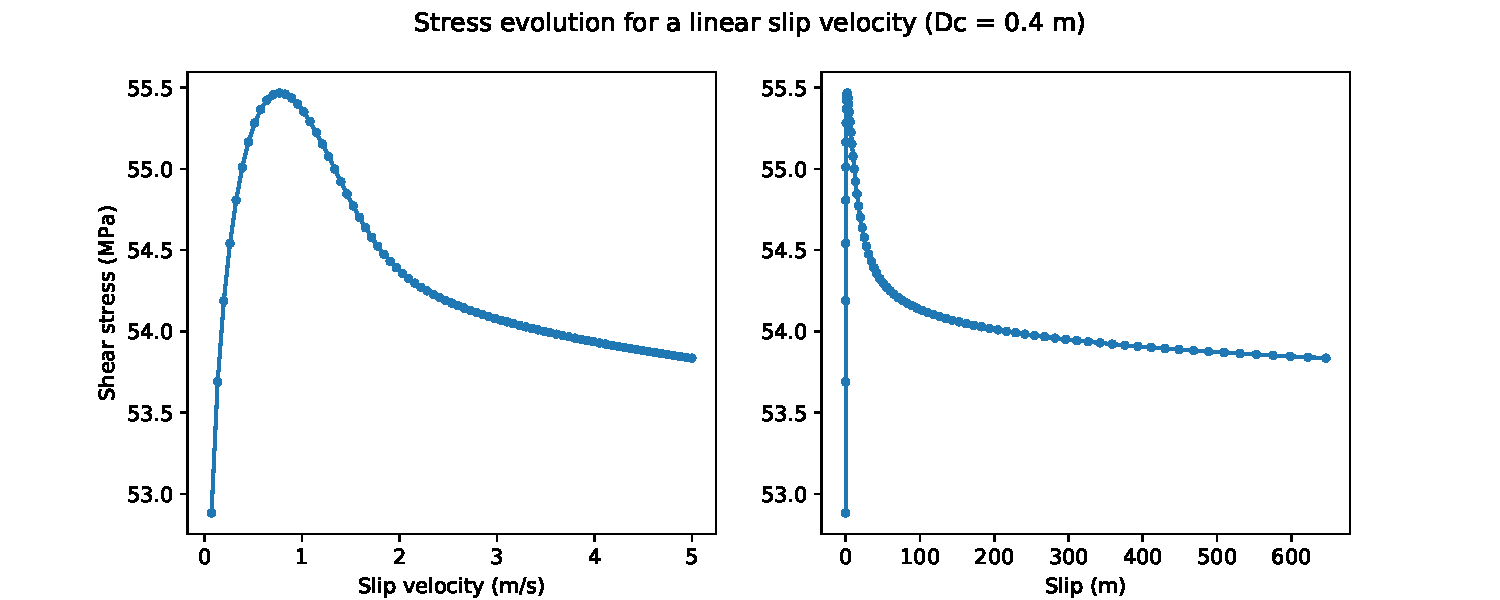
\includegraphics[scale=0.6]{fig1.pdf}
    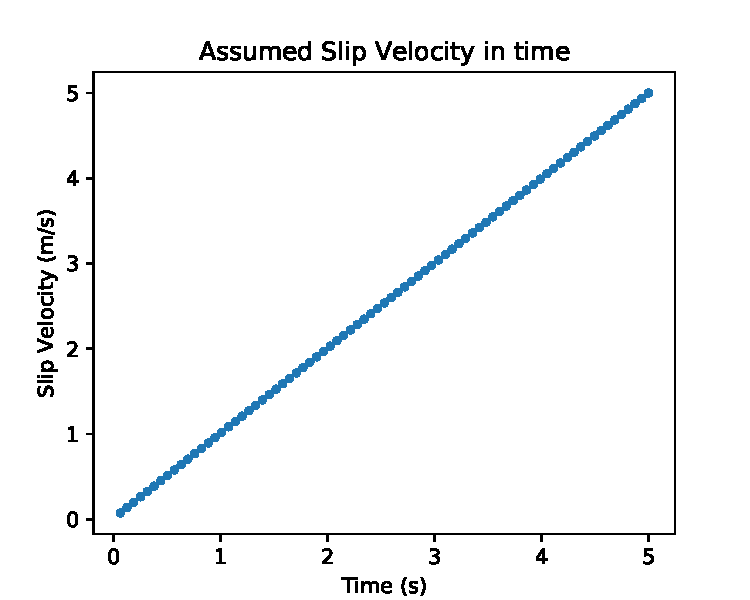
\includegraphics[scale=0.5]{fig1_v.pdf}
    \caption{The inferred slip weakening distance is around 60 m}
\end{figure}
\pagebreak
\begin{figure}[!htb]
    \centering
    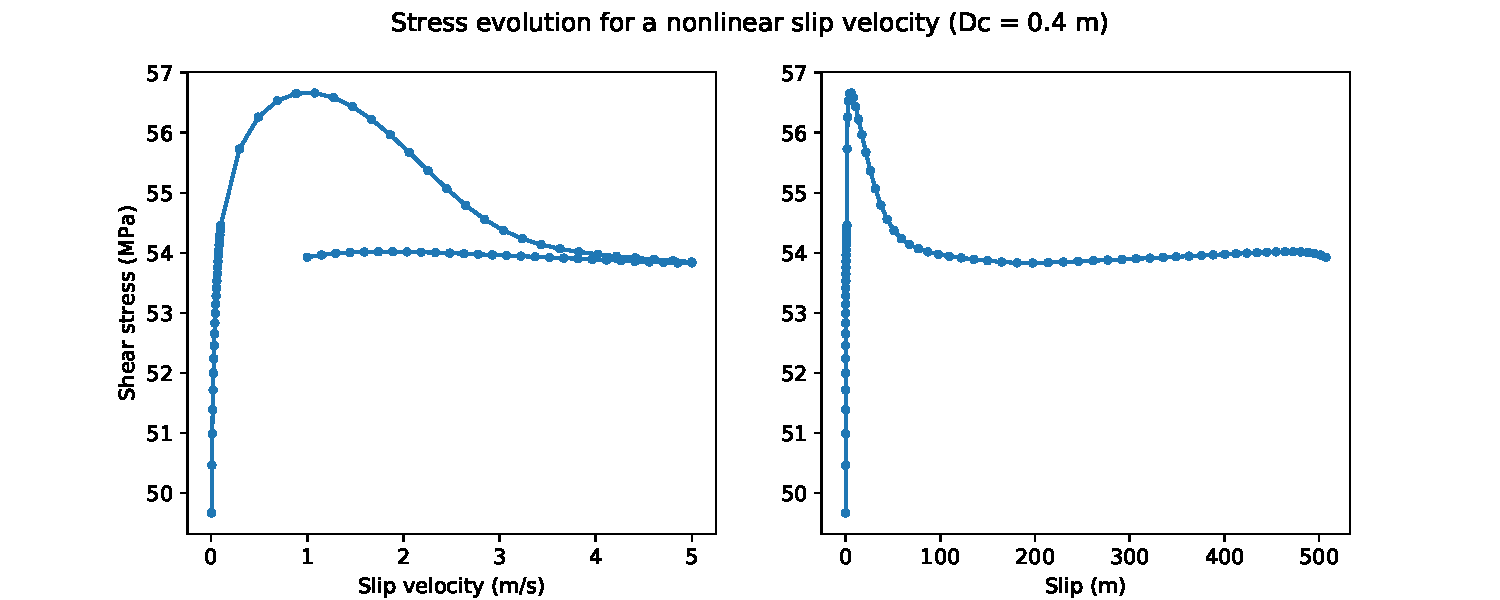
\includegraphics[scale=0.6]{fig2.pdf}
    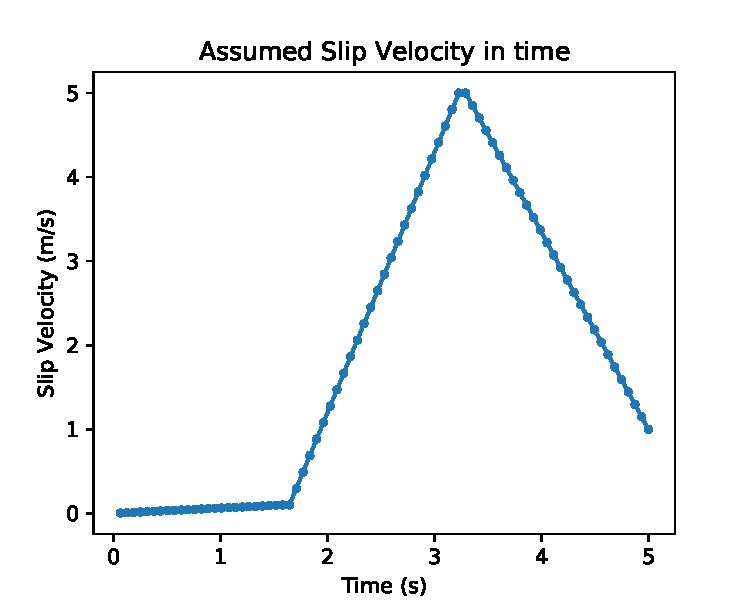
\includegraphics[scale=0.5]{fig2_v.pdf}
    \caption{The inferred slip weakening distance is around 80 m}
\end{figure}
\pagebreak
\begin{figure}[!htb]
    \centering
    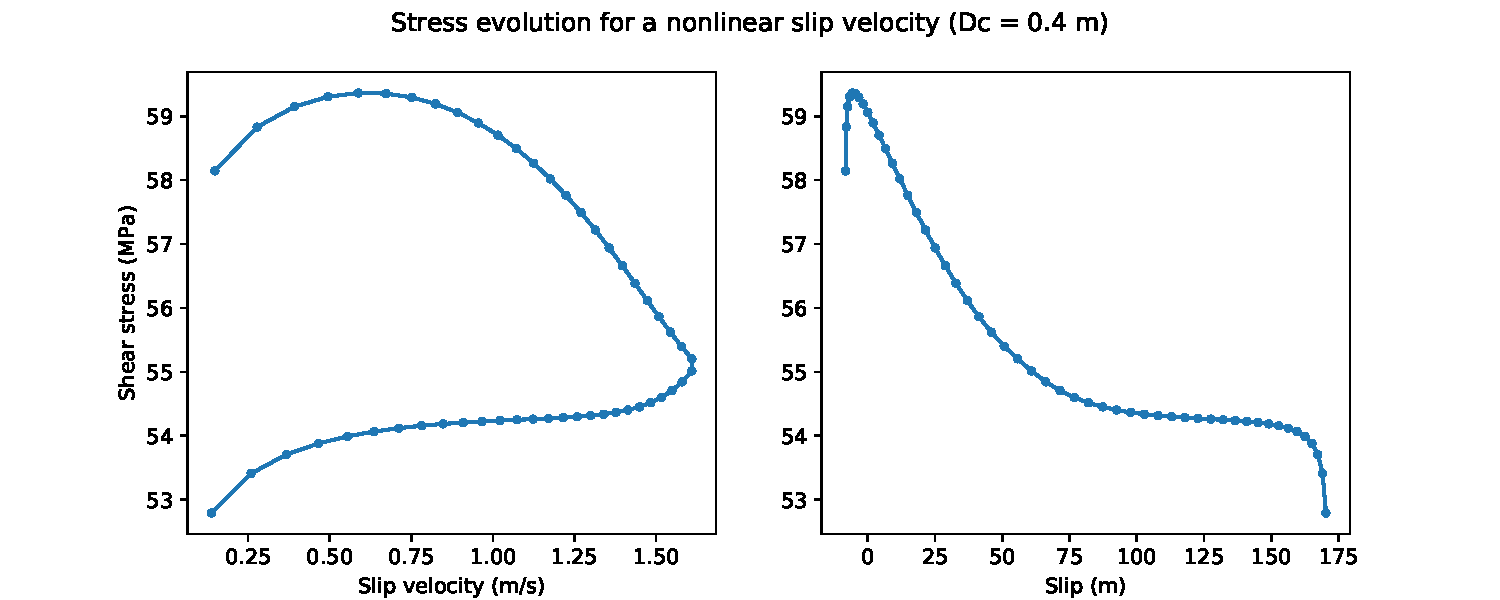
\includegraphics[scale=0.6]{fig3.pdf}
    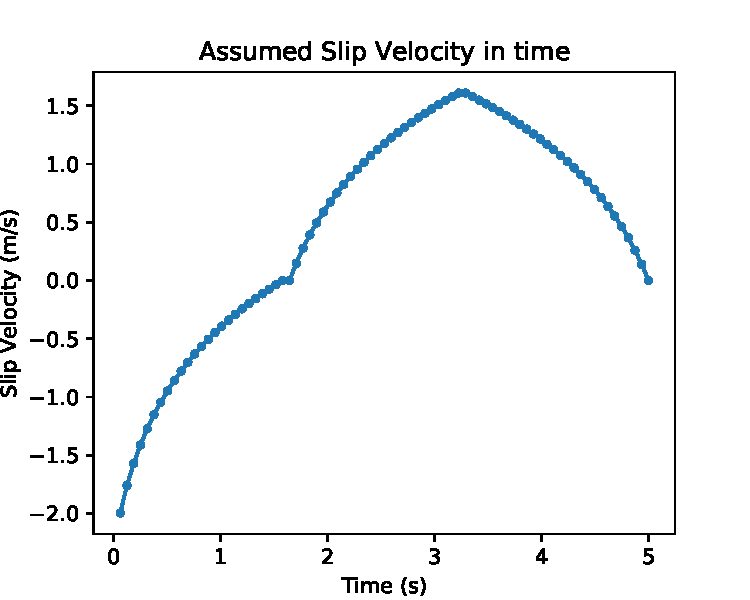
\includegraphics[scale=0.5]{fig3_v.pdf}
    \caption{The inferred slip weakening distance is around 75 m}
\end{figure}

\clearpage
\section*{Conclusions}
We see that the slip weakening law is a special case of rate and state friction law and by approximating the velocity as different set of functions, we can observe the slip weakening behavior. In the present exercise, we still see a very large slip weakening critical distance because the rate and state distance $D_c$ is large and the timesteps required are large in order for the numerical procedure to converge. Better initial velocity estimates are required to emulate the slip weakening behavior more accurately. 

\end{document}
